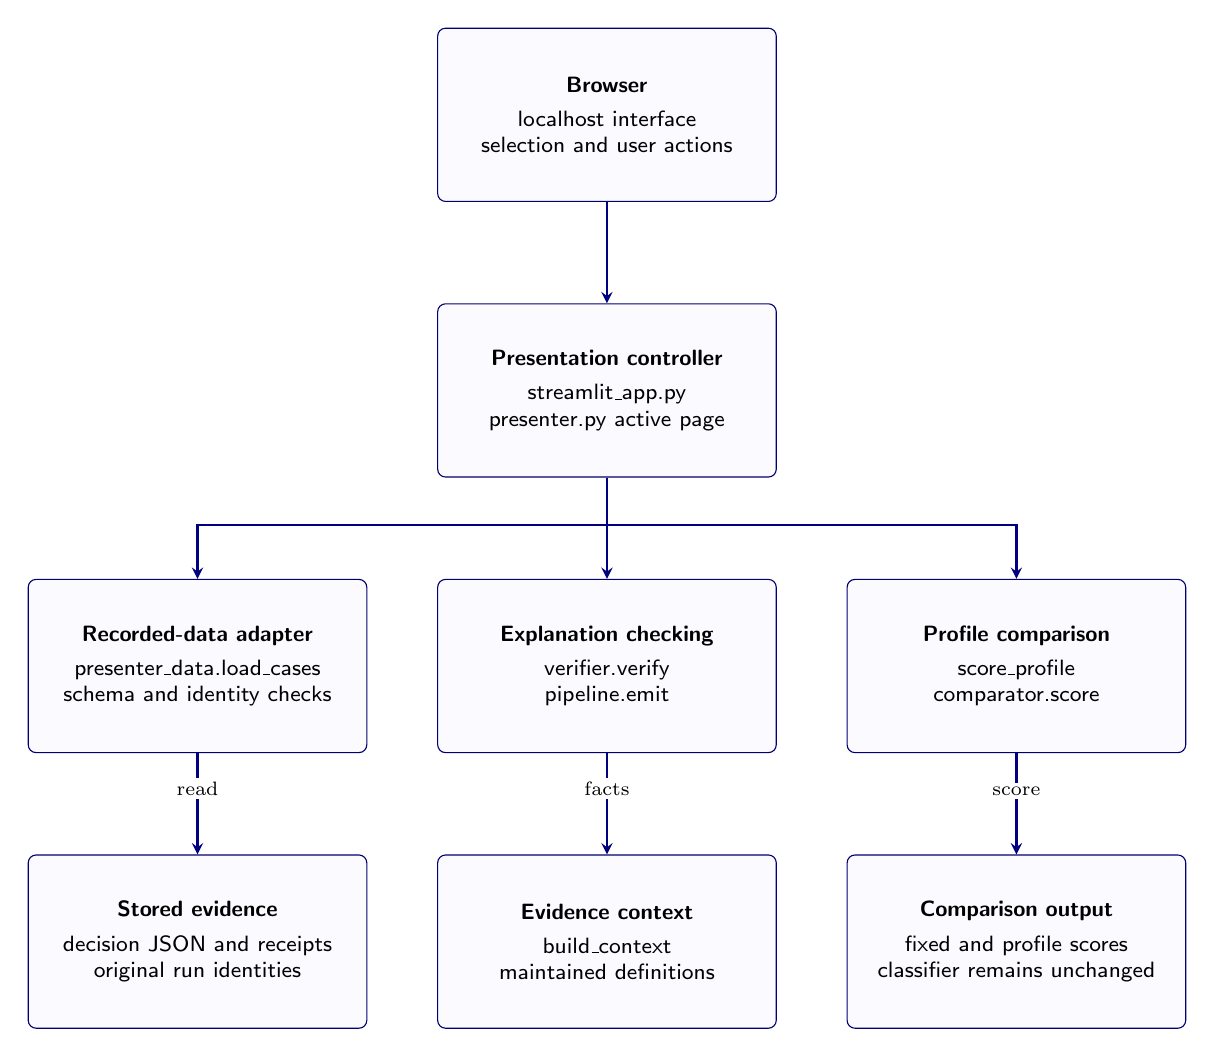
\begin{tikzpicture}[x=1mm,y=1mm,box/.style={draw=blue!45!black,fill=blue!2,rounded corners=1mm,align=center,text width=39mm,minimum height=22mm,inner sep=2mm,font=\sffamily\footnotesize},link/.style={->,>=stealth,draw=blue!50!black,thick}]
\node[box] (browser) at (75,140) {\textbf{Browser}\\[1mm]localhost interface\\selection and user actions};
\node[box] (presenter) at (75,105) {\textbf{Presentation controller}\\[1mm]streamlit\_app.py\\presenter.py active page};
\node[box] (loader) at (23,70) {\textbf{Recorded-data adapter}\\[1mm]presenter\_data.load\_cases\\schema and identity checks};
\node[box] (checking) at (75,70) {\textbf{Explanation checking}\\[1mm]verifier.verify\\pipeline.emit};
\node[box] (risk) at (127,70) {\textbf{Profile comparison}\\[1mm]score\_profile\\comparator.score};
\node[box] (artifacts) at (23,35) {\textbf{Stored evidence}\\[1mm]decision JSON and receipts\\original run identities};
\node[box] (context) at (75,35) {\textbf{Evidence context}\\[1mm]build\_context\\maintained definitions};
\node[box] (result) at (127,35) {\textbf{Comparison output}\\[1mm]fixed and profile scores\\classifier remains unchanged};
\draw[link] (browser.south) -- ++(0,-6) -| (presenter.north);
\draw[link] (presenter.south) -- ++(0,-6) -| (loader.north);
\draw[link] (presenter.south) -- ++(0,-6) -| (checking.north);
\draw[link] (presenter.south) -- ++(0,-6) -| (risk.north);
\draw[link] (loader.south) -- ++(0,-6) -| (artifacts.north) node[pos=.5,above,fill=white,inner sep=.5mm,font=\scriptsize]{read};
\draw[link] (checking.south) -- ++(0,-6) -| (context.north) node[pos=.5,above,fill=white,inner sep=.5mm,font=\scriptsize]{facts};
\draw[link] (risk.south) -- ++(0,-6) -| (result.north) node[pos=.5,above,fill=white,inner sep=.5mm,font=\scriptsize]{score};
\end{tikzpicture}
